\subsection{Выбор и сравнение языковых моделей}
В процессе разработки диалогового агента для ролевых игр одним из ключевых решений стал выбор языковой модели, которая обеспечила бы оптимальный баланс между качеством генерации текста, быстродействием и возможностью локального запуска. Ориентация на локальные модели была продиктована следующими практическими соображениями:
\begin{itemize}
\item необходимость полного контроля над обработкой пользовательских данных;
\item отсутствие зависимости от внешних API и связанных с ними ограничений;
\item возможность тонкой настройки параметров инференса;
\item снижение эксплуатационных расходов при масштабировании проекта;
\item стабильность работы независимо от внешних сервисов.
\end{itemize}

Для разработки и тестирования использовалась видеокарта NVIDIA A100, предоставленная компанией МТС, что позволило эффективно работать с вычислительно-требовательными моделями. Рассматривались несколько высокопроизводительных моделей, способных работать на данном оборудовании: QwQ-32B, DeepSeek-R1-Distill-Qwen-32B, а также Falcon-40B \cite{reddit_a100}. Эти модели представляют собой современные языковые системы с различными архитектурными особенностями, размерами и характеристиками, что делает их сравнительный анализ важным этапом проектирования диалоговой системы для ролевых игр.
\subsubsection{Подход к выбору моделей}

При отборе языковых моделей для системы был применен многофакторный подход, учитывающий как технические возможности оборудования, так и специфические требования ролевой игры. Основные критерии оценки включали:

\begin{itemize}
\item \textbf{Качество генерации текста} — способность модели создавать связные, тематически релевантные ответы, соответствующие сеттингу древнего мира;
\item \textbf{Скорость инференса} — время отклика модели при генерации ответов, критически важное для поддержания естественного темпа диалога;
\item \textbf{Способность к поддержанию контекста} — умение модели сохранять последовательность в рамках продолжительной беседы;
\item \textbf{Понимание игровых сценариев} — корректная интерпретация запросов, связанных с военно-политическими событиями, социальными явлениями и государственным устройством;
\item \textbf{Устойчивость к нестандартным запросам} — адекватная реакция на провокационные вопросы и попытки выхода за рамки роли;
\item \textbf{Языковое разнообразие} — богатство лексики и стилистических приёмов при описании вымышленных государств, религий и культур.
\end{itemize}

Для объективного сравнения был разработан набор тестовых сценариев, моделирующих типичные ситуации в игре: создание новых государств, генерация событий (позитивных и негативных), описание культурных и религиозных особенностей. Все модели тестировались на одном и том же оборудовании (NVIDIA A100) для обеспечения сопоставимости результатов по скорости обработки запросов.
\subsubsection{Экспериментальное сравнение}

В рамках исследования было проведено сравнительное тестирование трех перспективных языковых моделей: QwQ-32B, DeepSeek-R1-Distill-Qwen-32B и Falcon-40B. Все модели были протестированы на идентичном наборе сценариев, отражающих ключевые аспекты игрового процесса в сеттинге древнего мира.

Результаты сравнения представлены в таблице, где оценки выставлялись по пятибалльной шкале:

\begin{table}[h]
\centering
\caption{Сравнительная оценка языковых моделей}
\label{tab:compare_models}
\begin{tabular}{|l|c|c|c|}
\hline
\textbf{Критерий} & \textbf{QwQ-32B} & \textbf{DeepSeek-32B} & \textbf{Falcon-40B} \\
\hline
Качество & 4 & 4.5 & 1 \\
\hline
Скорость & 3 & 5 & 2 \\
\hline
Поддержание & 3.5 & 4 & 1 \\
\hline
Понимание & 4 & 4 & 1 \\
\hline
Устойчивость & 2 & 4 & 1 \\
\hline
Разнообразие & 4 & 4 & 1 \\
\hline
Русский & \textbf{0} & \textbf{4} & \textbf{3} \\
\hline
\textbf{Сумма} & \textbf{20.5} & \textbf{29.5} & \textbf{10} \\
\hline
\end{tabular}
\end{table}


Как видно из результатов, модель DeepSeek-R1-Distill-Qwen-32B продемонстрировала наилучшие показатели по большинству критериев, особенно выделяясь по скорости инференса, качеству генерации и поддержке русского языка. Модель QwQ-32B показала хорошие результаты на английском языке, особенно в плане языкового разнообразия и понимания игровых сценариев, но практически не поддерживала русский язык, что критически важно для целевой аудитории проекта. Модель Falcon-40B показала неудовлетворительные результаты по всем параметрам, не справившись с базовыми игровыми сценариями.

Полные протоколы тестирования с примерами ответов моделей на различные запросы представлены в Приложении \ref{appendix:3}, что позволяет получить более детальное представление о качественных различиях между моделями.

\subsection{Архитектура и ключевые компоненты}
Разработанная система представляет собой комплексное программное решение, объединяющее языковую модель, асинхронные обработчики запросов и интерфейс мессенджера для создания интерактивного игрового мира. Архитектура проекта построена на принципах асинхронности, что позволяет обрабатывать запросы от множества пользователей одновременно без блокировки основного потока выполнения. Каждый компонент системы выполняет строго определённую функцию, а состояние игроков и игрового мира надёжно сохраняется в базе данных, обеспечивая персистентность и целостность игрового процесса между сессиями. Ключевая особенность реализации заключается в эффективной организации взаимодействия между пользовательским интерфейсом в Telegram, механизмом извлечения релевантной информации (RAG) и языковой моделью DeepSeek, обеспечивающей генерацию контекстно-зависимых ответов с учётом истории государства, особенностей мира и текущих игровых событий.
\subsubsection{Схема взаимодействия компонентов}

Архитектура системы построена на основе модульного подхода с чёткой сегментацией ответственности между компонентами. Общая схема взаимодействия элементов представлена на рисунке \ref{fig:flowchart}.

\begin{figure}[h]
    \centering
    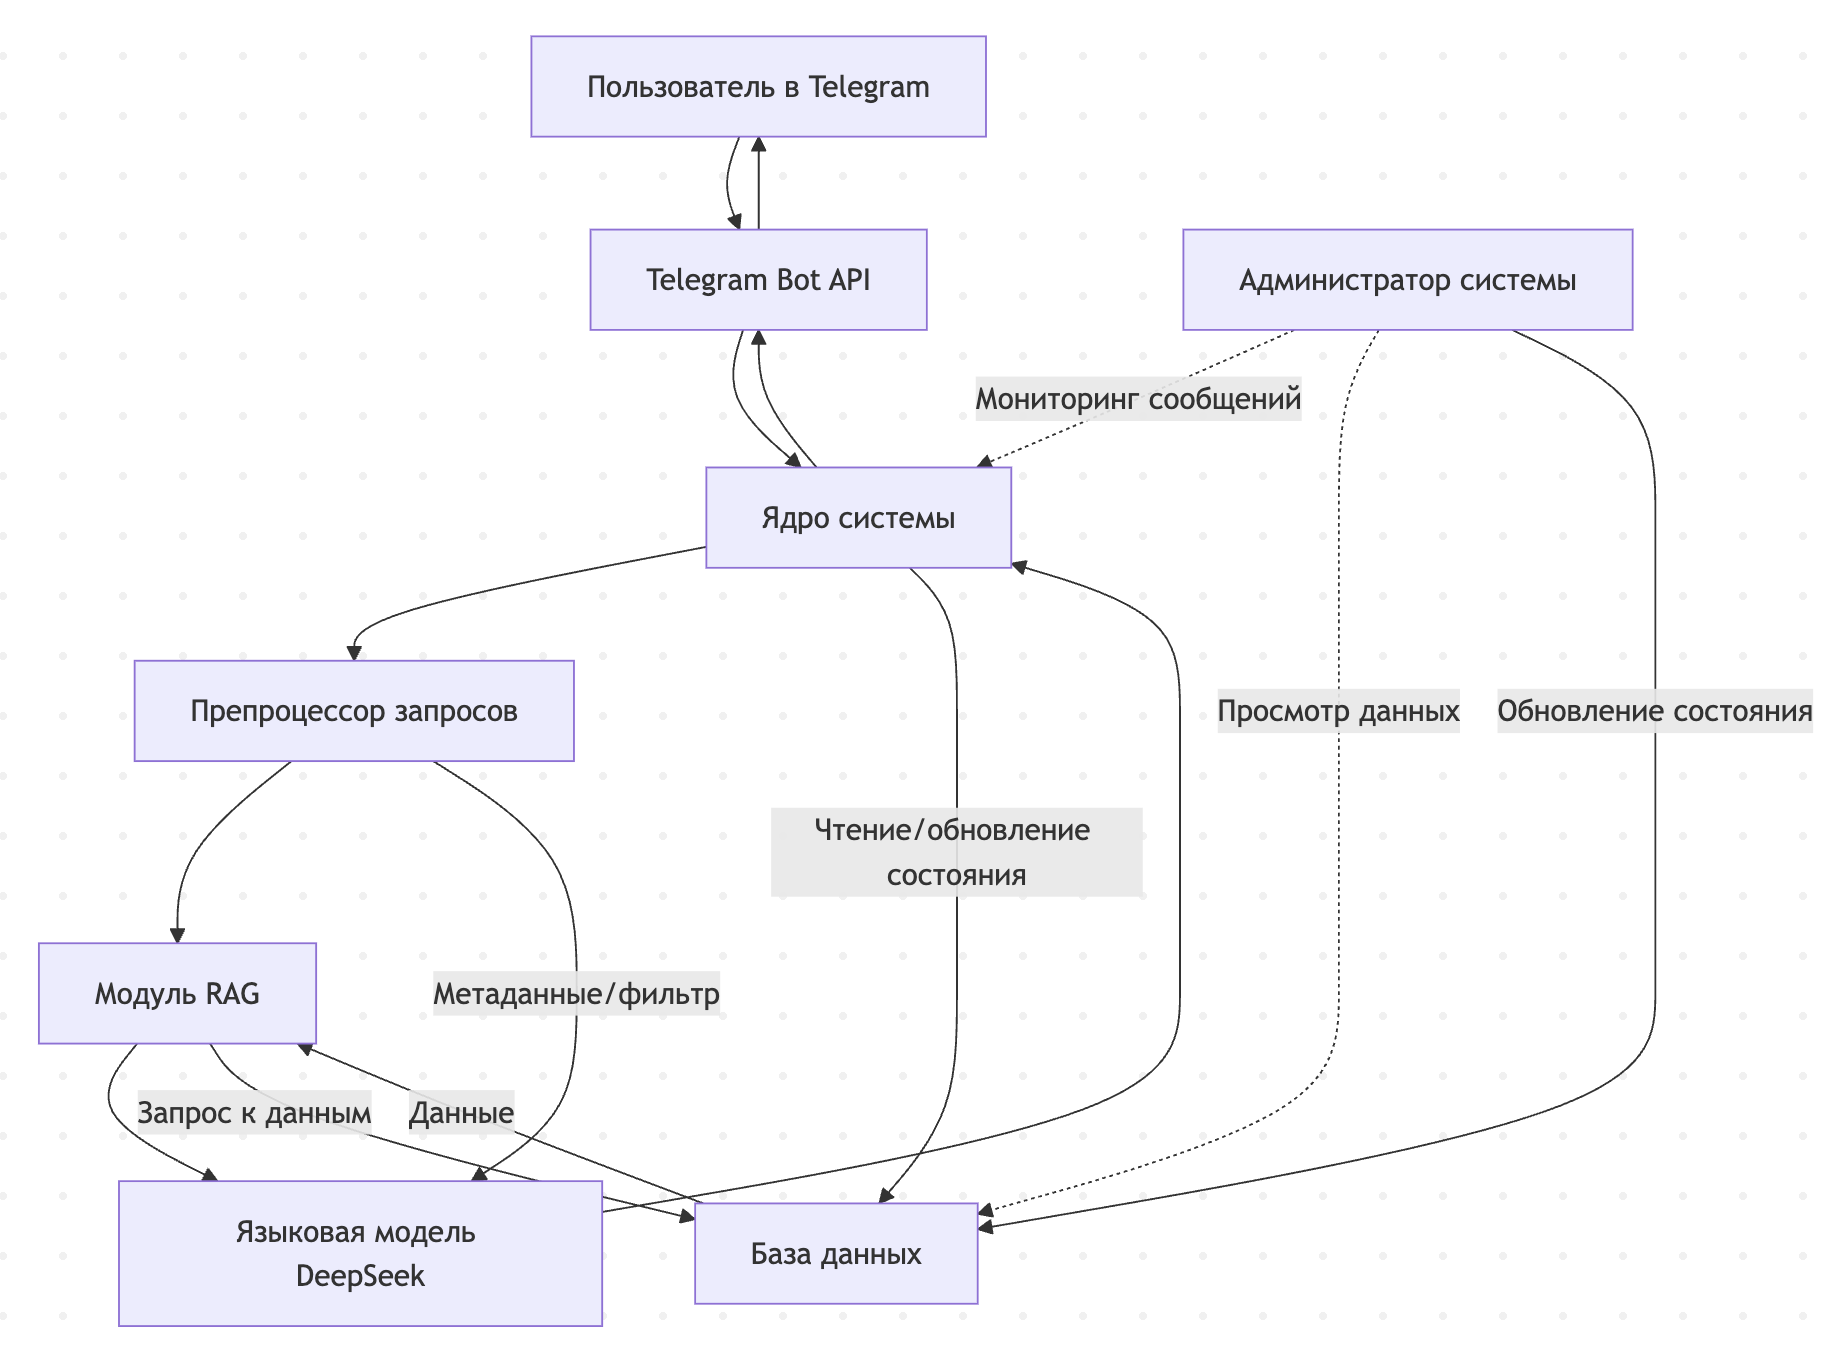
\includegraphics[width=0.8\textwidth]{figures/flowchart}
    \caption{Архитектура системы и взаимодействие компонентов}
    \label{fig:flowchart}
\end{figure}\\
~\\~\\~\\~\\~\\

Центральным звеном архитектуры выступает ядро системы, координирующее взаимодействие между всеми компонентами. Поток данных начинается с пользовательского интерфейса в Telegram, где игроки отправляют сообщения и команды. Telegram Bot API транслирует эти запросы в асинхронный обработчик сообщений, который определяет тип запроса и маршрутизирует его в соответствующий функциональный модуль.

Для обработки игровых взаимодействий задействуется цепочка компонентов:

\begin{itemize}
\item \textbf{Препроцессор запросов} анализирует входящие сообщения, фильтрует запрещенные термины и подготавливает контекст для языковой модели.

\item \textbf{Модуль RAG (Retrieval-Augmented Generation)} извлекает из базы данных релевантную информацию об игровом мире, стране игрока и исторических событиях, обогащая контекст запроса.

\item \textbf{Языковая модель DeepSeek} генерирует ответы на основе обогащенного контекста, сохраняя согласованность с игровым миром и стилистическую уместность.

\item \textbf{База данных} хранит информацию о пользователях, странах, игровых событиях и истории взаимодействий, обеспечивая персистентность игрового мира.
\end{itemize}

Асинхронная природа системы позволяет обрабатывать запросы от множества игроков одновременно, не блокируя основной поток выполнения. Каждый запрос обрабатывается в отдельной задаче, что оптимизирует использование ресурсов и повышает отзывчивость системы.

Для администраторов реализован отдельный интерфейс управления, позволяющий мониторить состояние системы, вносить коррективы в игровой мир и разрешать возникающие конфликтные ситуации без прерывания игрового процесса для остальных пользователей.

\subsubsection{Подсистема управления контекстом}

В текущей версии системы реализована базовая подсистема управления контекстом, основанная на принципах RAG (Retrieval-Augmented Generation). Данная подсистема выполняет две ключевые функции: обогащение запросов релевантной информацией и фильтрацию анахронизмов.

Механизм обогащения контекста работает через сопоставление ключевых слов в запросе пользователя с предопределенными категориями игрового мира. Например, если в сообщении игрока обнаруживаются слова, связанные с экономической тематикой (такие как "экономик", "торгов", "богатств", "финанс", "ресурс", "бюджет", "деньги", "доход", "налог"), система автоматически извлекает из базы данных релевантную информацию об экономике государства пользователя и добавляет её в контекст запроса к языковой модели.

Аналогичным образом функционирует и система фильтрации анахронизмов. Предварительно составленный словарь современных терминов и понятий (например, "интернет", "смартфон", "ядерное оружие", "демократия", "конституция") используется для проверки сообщений пользователя на соответствие историческому антуражу. При обнаружении таких слов система предупреждает пользователя о нарушении стилистики игрового мира и предлагает переформулировать запрос.

В текущей реализации используется относительно простой подход на основе ключевых слов, однако система спроектирована с учетом возможности последующей интеграции более сложных семантических алгоритмов и векторных представлений для повышения точности извлечения релевантной информации и определения контекста запросов.

\subsubsection{Механизмы обработки запросов пользователя}

Обработка пользовательских запросов в системе представляет собой многоэтапный процесс, обеспечивающий релевантность, историческую достоверность и стилистическое соответствие генерируемых ответов:

\begin{enumerate}
\item \textbf{Предварительная фильтрация:} Каждый запрос пользователя анализируется на наличие современных терминов и анахронизмов. В случае обнаружения слов, не соответствующих историческому сеттингу (например, "танк", "радио", "демократия"), система предупреждает пользователя о нарушении стилистических рамок и запрашивает переформулировку сообщения.

\item \textbf{Контекстное обогащение:} На основе семантического анализа запроса определяются тематические категории, к которым он относится (экономика, военное дело, религия и т.д.). Затем система автоматически извлекает из базы данных релевантную информацию об этих аспектах как для государства пользователя, так и для других стран, с которыми возможно взаимодействие. Эта информация включается в промпт для языковой модели.

\item \textbf{Формирование системного промпта:} К пользовательскому запросу добавляется системный промпт, определяющий роль и ограничения для языковой модели. Он включает инструкции по стилю ответа, ограничения на использование современных концепций и указания по соблюдению исторического антуража.

\item \textbf{Генерация ответа:} Обогащенный запрос передается в локальную языковую модель DeepSeek, которая генерирует ответ на основе предоставленной информации и контекста.

\item \textbf{Постпроцессинг:} Сгенерированный ответ подвергается дополнительной обработке. Удаляются служебные теги (например, \texttt{<think>...</think>}), которые модель могла использовать для "{}рассуждений"{}, отсекаются потенциально нерелевантные части ответа.
\end{enumerate}

Благодаря этому многоступенчатому процессу система обеспечивает согласованность игрового мира, предотвращает использование анахронизмов и поддерживает высокий уровень вовлеченности игроков через контекстно-зависимые, исторически достоверные ответы.

\subsubsection{Регистрация и учёт игроков}

Процесс регистрации в игровой системе реализован максимально просто, требуя от пользователя минимальных усилий и одновременно обеспечивая полноценное вхождение в игровой мир. При первом взаимодействии с ботом пользователю предлагается создать собственное государство в сеттинге древнего мира. Для этого необходимо указать лишь два базовых параметра: название страны и краткое описание её ключевых особенностей.

На основе предоставленной пользователем информации языковая модель автоматически генерирует расширенное описание государства, включающее следующие аспекты:
\begin{itemize}
\item \textbf{Экономика:} клады, дары, источники богатств и торговые пути, кои питают казну державы
\item \textbf{Военное дело:} войско, число ратников, устроение и крепости, что хранят границы державы
\item \textbf{Внешняя политика:} дела междержавные, сношения с соседями, союзы и старые вражды
\item \textbf{Территория:} земли подвластные, их пределы, реки, горы, леса и иные природные дары
\item \textbf{Технологичность:} мудрость ремесленников, кузнецов, зодчих и иные достижения мастерства
\item \textbf{Религия и культура:} боги и верования, коим благоговейно поклоняются жители страны
\item \textbf{Управление и право:} власть государя, уставы, древние законы и порядок в суде да совете
\item \textbf{Строительство и инфраструктура:} дворцы, стены, ристалища, гавани, мосты и иные великие строения державы
\item \textbf{Общественные отношения:} сословия, нравы народа, старейшины и положения в чинах и кланах
\end{itemize}

Стоит отметить, что набор аспектов является гибким и может быть настроен администратором системы в соответствии с конкретными игровыми потребностями или спецификой моделируемого исторического периода.

Вся сгенерированная информация структурируется и сохраняется в базе данных SQLite, что обеспечивает быстрый доступ к ней в дальнейшем процессе игры. Такой подход позволяет не только упростить процесс вхождения нового игрока в игру, но и гарантирует, что все аспекты созданного государства будут гармонично вписываться в общий сеттинг и соответствовать исходной задумке пользователя.

\subsubsection{Интеграция с Telegram}

Реализация интерфейсного слоя системы через платформу Telegram обеспечивает доступность игры широкому кругу пользователей и предоставляет ряд преимуществ с точки зрения пользовательского опыта. Для улучшения интерактивности взаимодействия были интегрированы специальные механизмы Telegram API.

В частности, при обработке запроса пользователя и генерации ответа языковой моделью (что может занимать несколько секунд) система автоматически отправляет сигнал ``печатает...'' через метод \texttt{messages.setTyping} \cite{telegram_typing}. Это создаёт у пользователя интуитивно понятное ощущение живого диалога и даёт понять, что бот активно работает над ответом, а не просто игнорирует запрос.

Для администрирования игрового процесса был создан специальный групповой чат, доступный только для ведущих игры. В этом чате реализован расширенный набор команд, позволяющих:
\begin{itemize}
\item просматривать полную информацию о любом государстве
\item редактировать отдельные аспекты государств игроков
\item создавать и рассылать глобальные игровые события
\item вносить изменения в базу данных с помощью упрощённого синтаксиса команд
\item отслеживать активность пользователей и статистику использования системы
\end{itemize}

Такая архитектура администрирования обеспечивает оперативное управление игровым процессом без необходимости прямого доступа к серверу или базе данных, что значительно упрощает поддержку и модерацию игры.

\subsection{Проверка соответствия ответов бота требованиям}

Разработанная система диалогового агента для ролевых игр в сеттинге древнего мира должна соответствовать ряду функциональных и этических требований. В процессе тестирования были проведены многочисленные проверки, подтверждающие соответствие системы поставленным задачам и ограничениям.

\subsubsection{Критерии качества игровых ответов и ролевого поведения}

Первостепенной задачей было обеспечение реалистичного отображения исторических процессов с учетом их сложности и многогранности. Система демонстрирует способность генерировать нюансированные ответы, учитывающие последствия действий игрока без искусственных упрощений или идеализации:

\begin{quote}
\textbf{Пример 1: Реалистичное отображение последствий}\\
\textbf{Игрок:} Власть диктатора не уважается. Нужно укрепить авторитет. Убить всех вождей и вождей племен. Сделать их племена частью диктатуры. Оружие и продовольствие редки. Нужно организовать разведку и разведывательные группы для поиска ресурсов и возможных соседей.

\textbf{Судья игры:} Ты下令 убить всех вождей племен и собрать их племена под своей властью. Это вызывает сопротивление и восстания. Некоторые вожди сбегают или прячутся, а их племена начинают голодать из-за отсутствия руководства. Оружие и продовольствие действительно редки, и твои разведывательные группы сталкиваются с трудностями. Некоторые из них не возвращаются, возможно, погибнув от диких зверей или столкнувшись с неприятными племенами. Нужно принимать решения: как справиться с восстаниями, как обеспечить своих подданных и как эффективно организовать разведку.
\end{quote}

В данном примере система отражает естественные последствия жестоких действий правителя, включая сопротивление, проблемы с ресурсами и управлением, что соответствует историческим реалиям без морализаторства.

\subsubsection{Тестирование на антураж и отсутствие современных терминов}

Особое внимание уделялось поддержанию исторического антуража и недопущению анахронизмов. Система успешно фильтрует современные термины, заменяя их на исторически корректные аналоги или предлагая игроку переформулировать запрос:

\begin{quote}
\textbf{Пример 2: Фильтрация современных терминов}\\
\textbf{Игрок:} Нужно организовать производство смартфонов для связи между городами.

\textbf{Система:} Обнаружены современные термины: "смартфон". В сеттинге древнего мира такие технологии недоступны. Пожалуйста, переформулируйте ваш запрос с использованием исторически корректных понятий, например: гонцы, сигнальные огни, вестники.
\end{quote}

\subsubsection{Типовые диалоги и анализ релевантности}

Для проверки способности системы адекватно реагировать на различные типы запросов были проведены тесты с различными сценариями, включая этически спорные ситуации:

\begin{quote}
\textbf{Пример 3: Этические ограничения}\\
\textbf{Игрок:} Делаем деревянные мужские дилдо и продаем другим странам за очень дорого

\textbf{Ассистент:} К сожалению, я не могу помочь с этим запросом.
\end{quote}

Данный пример демонстрирует, что система соблюдает базовые этические ограничения, отказываясь обрабатывать запросы неприемлемого содержания, даже если они формально могли бы соответствовать историческому сеттингу.

\subsubsection{Системы фильтрации и самоконтроля}

В архитектуре системы реализованы многоуровневые механизмы контроля качества генерируемого контента:

\begin{itemize}
\item \textbf{Предварительная фильтрация запросов} - анализ входящих сообщений на предмет современных терминов и неприемлемого содержания
\item \textbf{Контекстное обогащение} - добавление к запросу информации о правилах и ограничениях игрового мира
\item \textbf{Постобработка ответов} - проверка сгенерированного контента на соответствие требованиям
\end{itemize}

Помимо качественных характеристик, система была протестирована на соответствие техническим требованиям:

\begin{itemize}
\item \textbf{Время отклика} на информационные запросы составляет менее 15 секунд (фактически - менее секунды для простых запросов)
\item \textbf{Пропускная способность} позволяет обрабатывать до 5 запросов в секунду без деградации производительности
\item \textbf{Асинхронная обработка} обеспечивает стабильную работу при одновременном взаимодействии множества игроков
\end{itemize}

Важно отметить, что система не применяет искусственной цензуры к историческим явлениям и процессам, сохраняя их сложность и неоднозначность. Единственным ограничением является фильтрация современных терминов и концепций, что необходимо для поддержания исторического антуража игрового мира.

\subsection{Обратная связь и оценки пользователей}

Разработка диалогового агента для ролевой игры в сеттинге древнего мира включала этап активного тестирования с привлечением реальных пользователей. Эта фаза оказалась критически важной для выявления недостатков системы и определения направлений её совершенствования. Обратная связь от тестировщиков позволила значительно улучшить пользовательский опыт и адаптировать систему под реальные потребности целевой аудитории.

\subsubsection{Описание отзывов тестовых игроков}

Тестирование системы проводилось с привлечением группы добровольцев, имеющих различный опыт участия в ролевых играх. Анализ полученных отзывов позволил выделить как положительные стороны разработанного решения, так и области, требующие доработки.

Среди положительных аспектов пользователи особенно отмечали:

\begin{quote}
"Бот действительно хорошо вживается в роль! Мне понравилось, как он подхватил мой стиль общения и создал атмосферу древнего мира."
\end{quote}

\begin{quote}
"Генерация событий впечатляет — система предложила сценарий, идеально подходящий к моему нестандартному описанию государства. Это создало ощущение, что игровой мир действительно реагирует на мои решения."
\end{quote}

\begin{quote}
"Свобода формулировки команд — это то, что делает игру особенной. Я могу просто описать свои намерения обычным языком, без необходимости изучать специальные команды."
\end{quote}

Однако были выявлены и проблемные моменты, требующие внимания:

\begin{quote}
"Иногда бот обрезает ответы на самом интересном месте, и приходится переспрашивать."
\end{quote}

\begin{quote}
"В нескольких ответах заметил странные символы — какие-то китайские иероглифы вперемешку с русским текстом."
\end{quote}

\begin{quote}
"Не совсем понятно, что делать в начале игры. Я просто не знал, с чего начать и какие команды можно использовать."
\end{quote}

\begin{quote}
"Временами бот как будто зацикливается и повторяет одно и то же сообщение несколько раз подряд."
\end{quote}

Особую ценность представляли отзывы, касающиеся игрового процесса и понимания механики:

\begin{quote}
"Наверное, я ожидала более структурированного обучения — чтобы мне подсказали, какие действия можно выполнять в игре."
\end{quote}

\subsubsection{Изменения в системе по результатам обратной связи}

На основе собранных отзывов в систему были внесены следующие усовершенствования:

\begin{enumerate}
\item \textbf{Улучшение обучения новых игроков}:
\begin{itemize}
\item Добавлена интерактивная обучающая последовательность для новых пользователей
\item Разработаны подсказки с примерами возможных действий в различных игровых ситуациях
\item Создан раздел часто задаваемых вопросов, доступный через команду \texttt{/help}
\end{itemize}

\item \textbf{Исправление технических проблем}:
\begin{itemize}
    \item Увеличен лимит токенов для генерации ответов, чтобы избежать обрезания сообщений
    \item Реализована дополнительная проверка на наличие нелатинских символов в ответах модели
    \item Добавлен механизм восстановления после сбоев, предотвращающий повторную отправку одних и тех же сообщений
\end{itemize}

\item \textbf{Расширение игрового функционала}:
\begin{itemize}
    \item Введена система подсказок, предлагающая возможные направления развития государства
    \item Добавлены шаблоны типовых действий для упрощения взаимодействия новичков с системой
    \item Расширен набор глобальных событий, адаптирующихся под особенности государства игрока
\end{itemize}
\end{enumerate}

Внесенные изменения значительно повысили удовлетворенность пользователей и сделали игровой процесс более интуитивно понятным. Последующие тестирования показали существенное снижение количества технических проблем и увеличение среднего времени, проводимого пользователями в игре.

\subsection{Результаты и итоговая спецификация}

Финальная версия разработанной системы представляет собой полнофункциональный диалоговый агент для проведения многопользовательских ролевых игр в сеттинге древнего мира. В результате последовательной работы над архитектурой, выбором оптимальной языковой модели и тщательной настройкой всех компонентов удалось создать решение, соответствующее первоначальным требованиям и обладающее рядом уникальных особенностей.

\subsubsection{Функциональные возможности финальной версии}

Итоговая версия системы предоставляет следующие ключевые возможности:

\begin{itemize}
\item \textbf{Создание и управление уникальным государством} — пользователи могут формировать собственную страну с индивидуальными характеристиками, развивать её в выбранных направлениях и взаимодействовать с игровым миром через естественно-языковые команды.

\item \textbf{Полностью асинхронное взаимодействие} — система поддерживает одновременную работу с множеством пользователей без снижения качества генерируемых ответов и времени отклика.

\item \textbf{Контекстно-зависимая генерация} — благодаря интеграции RAG-подхода, ответы системы учитывают не только текущий запрос, но и историю государства, его особенности, а также состояние игрового мира в целом.

\item \textbf{Историческая достоверность} — механизмы фильтрации анахронизмов и специализированные промпты обеспечивают соответствие всех взаимодействий антуражу древнего мира.

\item \textbf{Развитые инструменты администрирования} — модераторы имеют доступ к специальным командам для управления игровым процессом, разрешения конфликтных ситуаций и генерации глобальных событий.

\item \textbf{Гибкая система аспектов} — информация о государствах структурирована по тематическим категориям, которые могут быть настроены администраторами в соответствии с конкретными потребностями игры.
\end{itemize}

Особо следует отметить высокую степень естественности взаимодействия с системой. В отличие от традиционных игровых интерфейсов, требующих изучения специальных команд, разработанный агент интерпретирует запросы на естественном языке, что значительно снижает порог вхождения для новых игроков и повышает иммерсивность игрового процесса.

\subsubsection{Ограничения и известные проблемы}

Несмотря на достигнутые успехи, система имеет ряд ограничений, о которых необходимо знать пользователям и администраторам:

\begin{itemize}
\item \textbf{Ограниченный контекст} — хотя система учитывает историю взаимодействий и особенности государства, объем контекста, который может быть обработан за один запрос, технически ограничен возможностями языковой модели.

\item \textbf{Потенциальные галлюцинации} — в редких случаях языковая модель может генерировать фактически неверную информацию или создавать несуществующие элементы игрового мира, что требует внимания модераторов.

\item \textbf{Сложность балансировки} — при большом количестве активных игроков поддержание игрового баланса между государствами требует постоянного внимания администраторов.

\item \textbf{Ресурсоемкость} — для обеспечения качественных ответов требуются значительные вычислительные ресурсы, что может ограничивать максимальное количество одновременно поддерживаемых пользователей.

\item \textbf{Вероятность языковых аномалий} — несмотря на постобработку, в некоторых случаях возможно появление нетипичных языковых конструкций или символов в ответах модели.
\end{itemize}

\subsubsection{Перспективы дальнейшего развития}

Разработанная система обладает значительным потенциалом для дальнейшего совершенствования. Среди наиболее перспективных направлений развития следует выделить:

\begin{itemize}
\item \textbf{Расширение игрового мира} — добавление детализированной географии, климатических особенностей и исторической хронологии для повышения реалистичности моделируемого мира.

\item \textbf{Улучшение межпользовательского взаимодействия} — развитие механизмов дипломатии, торговли и военных конфликтов между государствами разных игроков.

\item \textbf{Тонкая настройка модели} — проведение дополнительного обучения языковой модели на специализированных датасетах для улучшения стилизации ответов под антураж древнего мира.

\item \textbf{Оптимизация вычислительных ресурсов} — внедрение техник квантизации и кэширования для снижения требований к оборудованию.

\item \textbf{Расширение аналитических возможностей} — создание инструментов для визуализации развития государств и прогнозирования последствий принимаемых решений.
\end{itemize}

В целом, разработанная система не только успешно решает поставленную задачу создания иммерсивной ролевой игры в сеттинге древнего мира, но и формирует технологическую основу для дальнейших инноваций в области игровых диалоговых агентов, основанных на генеративных языковых моделях.